
% Conquest of Tlalocan chapter ========================================
\chapter*{Conquest of Tlalocan}
\addcontentsline{toc}{chapter}{Conquest of Tlalocan}

\begin{flushright}
\parbox{0.8\textwidth}{
\emph{The human mind is inspired enough when it comes to inventing
horrors; it is when it tries to invent a Heaven that it shows itself
cloddish. \\
\hspace*{\fill}{\textperiodcentered \textperiodcentered \textperiodcentered \hspace*{0.2em} Evelyn Waugh} } }
\end{flushright}

\noindent
Conquest of Tlalocan is chess variant which is played on 24 x 24 board,
with bright red and cyan fields, and dark red and light green pieces.
Star colors are bright red and bright blue. In algebraic notation, columns
are enumerated from 'a' to 'x', and rows are enumerated from '1' to '24'.
A new piece is introduced, Shaman.

\clearpage % ..........................................................
% Shaman **************************************************************

\section*{Shaman}
\addcontentsline{toc}{section}{Shaman}

\noindent
\begin{wrapfigure}{l}{0.4\textwidth}
\centering
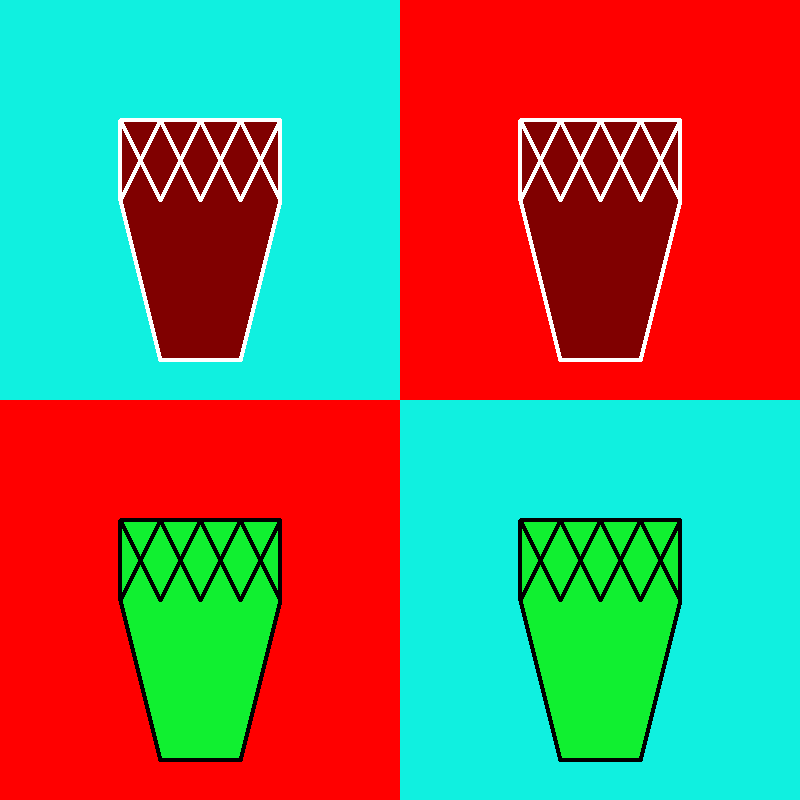
\includegraphics[width=0.4\textwidth, keepaspectratio=true]{pieces/14_shaman.png}
\caption{Shaman}
\label{fig:14_shaman}
\end{wrapfigure}


*** separate step-fields and capture-fields ***

Moves similar to Unicorn. For light Shaman, step-fields are as
Knight, capture-field are as long-range Unicorn. For dark one,
it's the opposite.

Trance-journey ...


% \vspace*{0.05\textheight}
\noindent
\begin{wrapfigure}{l}{0.4\textwidth}
\centering
\includegraphics[width=0.4\textwidth, keepaspectratio=true]{pieces/star/18_conquest_of_tlalocan.png}
\caption{Star}
\label{fig:star/18_conquest_of_tlalocan}
\end{wrapfigure}
Star colors in this variant are presented on the left.

% ************************************************************** Shaman
\clearpage % ..........................................................

\section*{Promotion}
\addcontentsline{toc}{section}{Promotion}

Promotion is non enforced, delayed variety, i.e. it's the same as in
\hyperref[sec:Age of Aquarius/Promotion]{previous chess variant}, Age of Aquarius.

Promotion in this variant is polygamous, more than one Queen in the same color
can be present on chessboard at any given time.

\clearpage % ..........................................................

\section*{En passant}
\addcontentsline{toc}{section}{En passant}

\noindent
\begin{wrapfigure}{l}{0.4\textwidth}
\centering
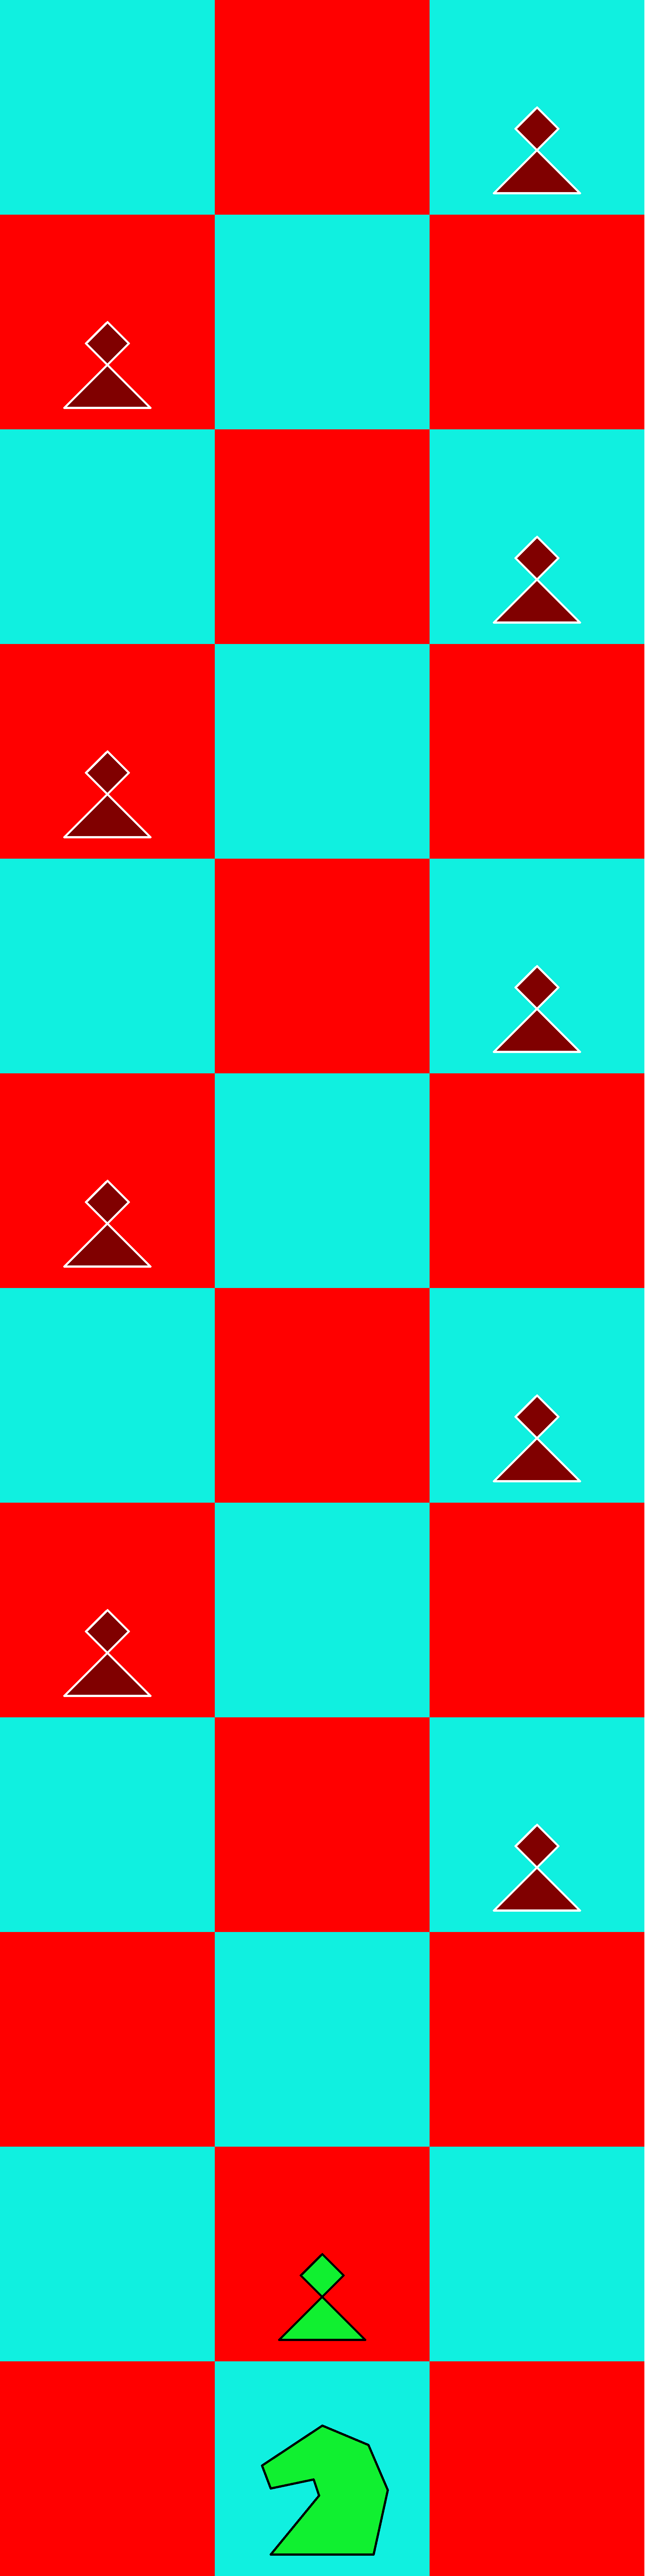
\includegraphics[width=0.125\textwidth, keepaspectratio=true]{en_passants/18_conquest_of_tlalocan_en_passant.png}
\caption{En passant}
\label{fig:18_conquest_of_tlalocan_en_passant}
\end{wrapfigure}
Rush and en passant are identical to those in Classic Chess, only difference
is that Pawn can now move longer on initial turn, up to 9 fields in this
variant.

\clearpage % ..........................................................

\section*{Castling}
\addcontentsline{toc}{section}{Castling}

Castling is the same as in Classical Chess, only difference is that King can move between 2 and 8 fields across.
All other constraints from Classical Chess still applies.

\noindent
\begin{figure}[!h]
% \begin{figure}[!t]
\includegraphics[width=1.0\textwidth, keepaspectratio=true]{castlings/18_cot/conquest_of_tlalocan_castling.png}
\caption{Castling}
\label{fig:conquest_of_tlalocan_castling}
% \centering
\end{figure}

In example above, all valid King's castling moves are numbered.

\noindent
\begin{figure}[!h]
% \begin{figure}[!t]
\includegraphics[width=1.0\textwidth, keepaspectratio=true]{castlings/18_cot/conquest_of_tlalocan_castling_right_08.png}
\caption{Castling long right}
\label{fig:conquest_of_tlalocan_castling_right_08}
% \centering
\end{figure}

In this example King was castling long to the right. Initial King's position is marked with "K".
After castling is finished, right Rook ends up at field immediately left to the King.

\clearpage % ..........................................................

\section*{Initial setup}
\addcontentsline{toc}{section}{Initial setup}

Compared to initial setup of Tamoanchan Revisited, Shaman is inserted between Unicorn and Pyramid
symmetrically, on both sides of chessboard. This can be seen in the image below:

\noindent
% \begin{figure}[t]
\begin{figure}[h]
\includegraphics[width=1.0\textwidth, keepaspectratio=true]{boards/18_conquest_of_tlalocan.png}
\caption{Conquest of Tlalocan board}
\label{fig:18_conquest_of_tlalocan}
% \centering
\end{figure}

\clearpage % ..........................................................
% ======================================== Conquest of Tlalocan chapter
